\documentclass[a4paper,12pt]{article}
\usepackage{amsmath,amssymb,amsfonts,amsthm}
\usepackage{tikz}
\usepackage [utf8x] {inputenc}
\usepackage [T2A] {fontenc} 
\usepackage[russian]{babel}
\usepackage{cmap, upgreek}
\usepackage{textcomp} 

% Так ссылки в PDF будут активны
\usepackage[unicode]{hyperref}

% вы сможете вставлять картинки командой \includegraphics[width=0.7\textwidth]{ИМЯ ФАЙЛА}
% получается подключать, как минимум, файлы .pdf, .jpg, .png.
\usepackage{graphicx}
% Если вы хотите явно указать поля:
\usepackage[margin=1in]{geometry}
% Или если вы хотите задать поля менее явно (чем больше DIV, тем больше места под текст):
% \usepackage[DIV=10]{typearea}

\usepackage{fancyhdr}

\newcommand{\bbR}{\mathbb R}%теперь вместо длинной команды \mathbb R (множество вещественных чисел) можно писать короткую запись \bbR. Вместо \bbR вы можете вписать любую строчку букв, которая начинается с '\'.
\newcommand{\eps}{\varepsilon}
\newcommand{\bbN}{\mathbb N}
\newcommand{\dif}{\mathrm{d}}

\newtheorem{Def}{Определение}


\pagestyle{fancy}
\makeatletter % сделать "@" "буквой", а не "спецсимволом" - можно использовать "служебные" команды, содержащие @ в названии
\fancyhead[L]{\footnotesize Электричество и магнетизм}%Это будет написано вверху страницы слева
\fancyhead[R]{\footnotesize ФМХФ МФТИ}
\fancyfoot[L]{\footnotesize \@author}%имя автора будет написано внизу страницы слева
\fancyfoot[R]{\thepage}%номер страницы —- внизу справа
\fancyfoot[C]{}%по центру внизу страницы пусто

\renewcommand{\maketitle}{%
	\noindent{\bfseries\scshape\large\@title\ \mdseries\upshape}\par
	\noindent {\large\itshape\@author}
	\vskip 2ex}
\makeatother
\def\dd#1#2{\frac{\partial#1}{\partial#2}}


\title{3.2.1 \\ Сдвиг фаз в цепи переменного тока}
\author{Егор Берсенев} 
\date{15 апреля 2016 г.}

\begin{document}
	\maketitle
	\section{Цель работы}
		 Изучить влияние активного сопротивления, индуктивности и ёмкости на сдвиг фаз между током и напряжением в цепи переменного тока.
	\section{Оборудование}
		Генератор звуковой частоты, двухканальный осциллограф, магазин емкостей, магазин сопротивлений, катушка индуктивности, резисторы, мост переменного тока.
	\section{Теоретическая часть}
		Измерять сдвиг фаз в цепях переменного тока можно с помощью осицллографа. Пусть нужно измерить сдвиг фаз между двумя напряжениями $U_1$ и $U_2$. Подадим эти напряжения на соответсвующие входы осциллографа. Смещения луча определяются $$ x = x_0\cos\Omega t \qquad y = y_0\cos\left(\Omega t +\alpha\right) $$
		Исключим время
		$$ \left(\frac{x}{x_0}\right)^2 + \left(\frac{y}{y_0}\right)^2+\frac{2xy}{x_0y_0}\cos\alpha = \sin^2\alpha$$
		Это выражение определяет эллипс на экране осциллографа. Для расчёта сдвига фаз можно измерить отрезки $2y_{x=0}$ и $2y_0$ и, подставляя эти значения в уравнение эллипса, найдем
		$$\alpha = \pm\arcsin\left(\frac{y_{x=0}}{y_0}\right) $$.
		
		\includegraphics[width = 0.5\linewidth]{pic3}\label{pic1}
		
		На практике применяются фазовращатели, позволяющие в широких пределах изменять фазу напряжения. Этот прибор включает в себя два одинаковых резистора, емкость и реостат. Используя метод комплексных амплитуд, найдем зависимость сдвига фаз между входным и выходным напряжением в зависимости соотношения между импедансами сопротивления $R$ и ёмкости $C$. Для этого выразим выходное напряжение через параметры контура и частоту внешнего источника.
		
		\includegraphics[width = 0.3\linewidth]{pic1} 
		
		Пусть комплексная амплитуда входного напряжения $\hat{U_0}$. Тогда напряжение между точками 1 и 3 в силу равенства сопротивлений:
		$$\hat{U_{13}} = \frac{\hat{U_0}}{2}.$$
		Пусть фаза входного напряжения равна нулю, тогда $\hat{U_0}$ будет действительной величиной. Примем напряжение в точке 1 равным нулю, тогда:
		$$\hat{U_{03}} = \frac{U_0}{2}$$
		Рассчитаем амплитуду в точке 4. Импеданс последовательно соединенных емкости и сопротивления равен 
		$$Z = R - \frac{i}{\Omega C}.$$
		Для комплексной амплитуды тока $\hat{I_0|}$, проходящего через R и C, имеем
		$$\hat{I_0} = \frac{U_0}{Z}=\cfrac{U_0}{R-\cfrac{i}{\Omega C}},$$
		а для комплексной амплитуды напряжения в точке 4 ---
		$$ \hat{U_{04}} = \hat{I_0}R = U_0\cfrac{R}{R-\cfrac{i}{\Omega C}}$$
		Тогда выходное напряжение:
		$$ \hat{U_{\text{вых}}} = \hat{U_{04}}-\hat{U_{03}} = \hat{U_{04}}-\frac{U_0}{2} = \frac{U_0}{2}\cfrac{R+\cfrac{i}{\Omega C}}{R - \cfrac{i}{\Omega C}}.$$
			Величина выходного напряжения не меняется, посколько модули комплексных величин одинаковы. Сдвиг фаз равен $2\arctan\left(\frac{1}{\Omega RC}\right)$ и меняется от $\frac{\pi}{2}$ до $ 0$.
		\subsection{Экспериментальная установка}
		Экспериментальная установка:
		
		\includegraphics[width = 0.7\linewidth]{pic2}
		
		Установка для исследования фазовращателя:
		
		\includegraphics[width = 0.7\linewidth]{pic4}
	
	\section{Ход работы}
	\subsection{Измерение зависимости сдвига фаз от R в RC-цепи}
	$$ R = 12.2 \text{Ом}$$
	$$ f = 1000 \text{Гц}$$
	$$ \Omega = 6280 \text{рад/с} $$
	$$ C = 5\cdot 10^{-1} \text{Ф}$$
	\begin{table}[h]
		\centering
		\caption{Измерение зависимости сдвига фаз от R в RC-цепи}
		\label{my-label}
		\begin{tabular}{|l|l|l|l|l|l|l|l|}
			\hline
			$R$    & $x$   & $x_0$ & $f$, рад          & $\cot f$    & $RS$     & $\frac{1}{\Omega CR}$ & $\Omega CR$ \\ \hline
			0    & 5   & 10   & 1,571 & $6,13\cdot10^{-17}$ & 12,2   & 26,10  & 0,04 \\ \hline
			500  & 2,5 & 10   & 0,785 & 1,00     & 512,2  & 0,62   & 1,61 \\ \hline
			1000 & 1,5 & 10   & 0,471 & 1,96     & 1012,2 & 0,31   & 3,18 \\ \hline
			1500 & 1   & 10   & 0,314 & 3,08     & 1512,2 & 0,21   & 4,75 \\ \hline
			2000 & 0,8 & 10   & 0,251 & 3,89     & 2012,2 & 0,16   & 6,32 \\ \hline
			750  & 1,8 & 10   & 0,565 & 1,58     & 762,2  & 0,42   & 2,39 \\ \hline
			1250 & 1   & 10   & 0,314 & 3,08     & 1262,2 & 0,25   & 3,96 \\ \hline
			\end{tabular}
	\end{table}
	
	\includegraphics[width = 0.7\linewidth]{graph2}
		
	\subsection{Исследование зависимости сдвига фаз от R в RL-цепи}
	$$ R = 12.2\, \text{Ом}$$
	$$ f = 1000\, \text{Гц}$$
	$$ \Omega = 6280\, \text{рад/с} $$
	$$ L = 0.5024\, \text{мГн}$$
	
	\begin{table}[h]
		\centering
		\caption{Исследование зависимости сдвига фаз от R в RL-цепи}
		\label{my-label}
		\begin{tabular}{|l|l|l|l|l|l|l|l|}
			\hline
			$R$    & $x$   & $x_0$ & $f$ рад          & $\cot f$    & $RS$     & $\frac{\Omega L}{RS}$ & $\frac{RS}{\Omega L}$ \\ \hline
			0    & 6   & 10   & 1,885 & -0,325 & 44   & 71,706 & 0,014 \\ \hline
			400  & 2,5 & 10   & 0,785 & 1      & 444  & 7,106  & 0,141 \\ \hline
			800  & 1,5 & 10   & 0,471 & 1,963  & 844  & 3,738  & 0,268 \\ \hline
			1200 & 1   & 10   & 0,314 & 3,078  & 1244 & 2,536  & 0,394 \\ \hline
			1600 & 0,8 & 10   & 0,251 & 3,895  & 1644 & 1,919  & 0,521 \\ \hline
			1000 & 1,2 & 10   & 0,377 & 2,526  & 1044 & 3,022  & 0,331 \\ \hline
		\end{tabular}
		\end{table}
	
	\includegraphics[width = 0.65\linewidth]{graph4}
	
	\subsection{Теоретические графики}
	Сдвиг фаз в RL-цепи:
	
		\includegraphics[width = 0.9\linewidth]{graph3}
		
	Сдвиг фаз в RC-цепи:
	
		\includegraphics[width = 0.9\linewidth]{graph1}
		
	\pagebreak
	\subsection{Исследование зависимости сдвига фаз от частоты в RCL-цепи}
	Расчетная частота резонанса $f_0 = 1055\,\text{Гц},\,C = 5\cdot 10^{-1} \text{Ф},\,L = 0.5024\, \text{мГн}$.
	\begin{table}[h]
		\centering
		\caption{Исследование зависимости сдвига фаз от частоты в RCL-цепи, 1}
		\label{my-label}
		\begin{tabular}{|l|l|l|l|l|}
			\hline
			$f$    & $x$   & $x_0$ & $f$     & $\frac{f}{f_0}$ \\ \hline
			800  & 6   & 31   & 0,608 & 0,797  \\ \hline
			750  & 7   & 39,5 & 0,557 & 0,747  \\ \hline
			850  & 5,5 & 30   & 0,576 & 0,846  \\ \hline
			900  & 4,5 & 28   & 0,505 & 0,896  \\ \hline
			950  & 3   & 26,5 & 0,356 & 0,946  \\ \hline
			700  & 3   & 14,5 & 0,650 & 0,697  \\ \hline
			650  & 3,5 & 16   & 0,687 & 0,647  \\ \hline
			1040 & 2   & 24   & 0,262 & 1,036  \\ \hline
			1100 & 3,5 & 23   & 0,478 & 1,095  \\ \hline
			1140 & 4   & 22   & 0,571 & 1,135  \\ \hline
			1200 & 4   & 21   & 0,598 & 1,195  \\ \hline
			1240 & 4   & 20   & 0,628 & 1,235  \\ \hline
			1300 & 3   & 19   & 0,496 & 1,295  \\ \hline
		\end{tabular}
	\end{table}
	
	\begin{table}[h]
		\centering
		\caption{Исследование зависимости сдвига фаз от частоты в RCL-цепи, 2}
		\label{my-label}
		\begin{tabular}{|l|l|l|l|l|}
			\hline
			$f$    & $x$   & $x_0$ & $f$     & $\frac{f}{f_0}$ \\ \hline
			800  & 6   & 31   & 0,608 & 0,797  \\ \hline
			750  & 7   & 39,5 & 0,557 & 0,747  \\ \hline
			850  & 5,5 & 30   & 0,576 & 0,846  \\ \hline
			900  & 4,5 & 28   & 0,505 & 0,896  \\ \hline
			950  & 3   & 26,5 & 0,356 & 0,946  \\ \hline
			700  & 3   & 14,5 & 0,650 & 0,697  \\ \hline
			650  & 3,5 & 16   & 0,687 & 0,647  \\ \hline
			1040 & 2   & 24   & 0,262 & 1,036  \\ \hline
			1100 & 3,5 & 23   & 0,478 & 1,095  \\ \hline
			1140 & 4   & 22   & 0,571 & 1,135  \\ \hline
			1200 & 4   & 21   & 0,598 & 1,195  \\ \hline
			1240 & 4   & 20   & 0,628 & 1,235  \\ \hline
			1300 & 3   & 19   & 0,496 & 1,295  \\ \hline
		\end{tabular}
	\end{table}
	
	\includegraphics[width = 0.7\linewidth]{graph5}

	\begin{table}[h]
		\centering
		\caption{Результаты измерений}
		\label{my-label}
		\begin{tabular}{|l|l|l|}
			\hline
			$R$      & 0                & 100   \\ \hline
			$p_1$    & 0.948            & 0.929 \\ \hline
			$p_2$    & 1.062            & 1.081 \\ \hline
			$\dif p$ & 0.114            & 0.152 \\ \hline
			$Q$      & 8.74             & 6.59  \\ \hline
			$Q_t$    & $1.39\cdot 10^4$ & 6.752 \\ \hline
		\end{tabular}
	\end{table}
	
	\subsection{Векторная диаграмма}
	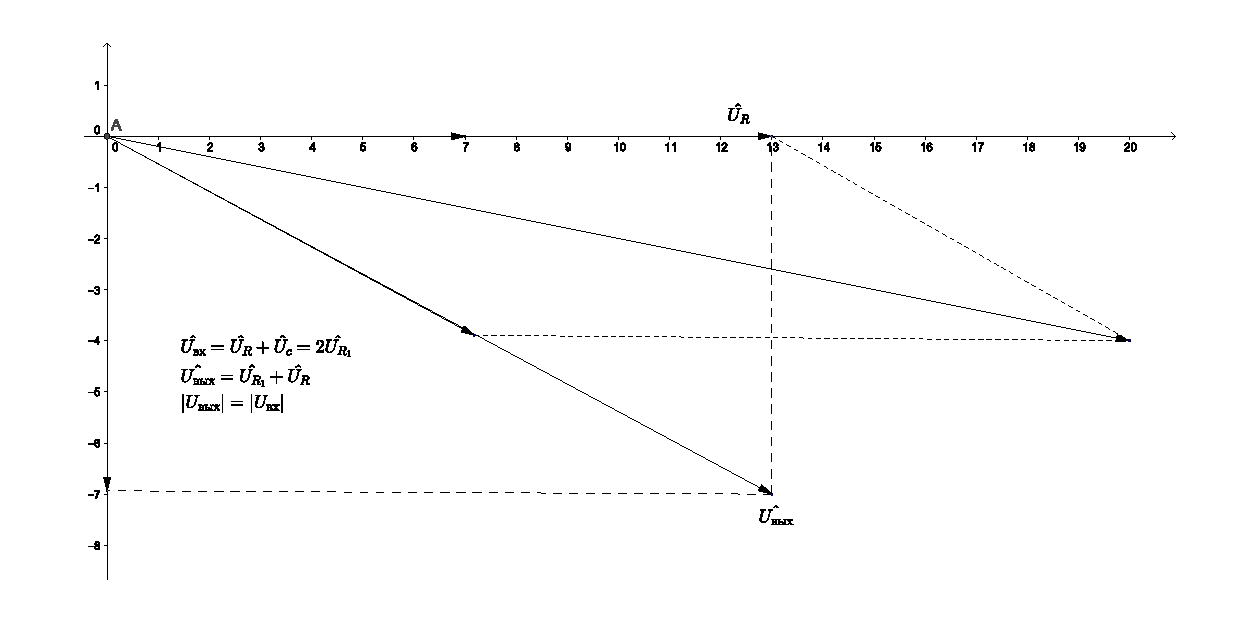
\includegraphics[width = 0.8\linewidth]{pic5}

	
	\section{Вывод} 
		В цепи переменного тока, содержащей емкости и индуктивности возникает разность фаз между током и напряжением. При включении индуктивности ток опережает напряжения, при включении емкости наоборот.
\end{document}


